\documentclass[ngerman,ruledheaders=section,class=report,thesis={type=Protokoll},accentcolor=1b,marginpar=false,parskip=half-,fontsize=11pt,]{tudapub}

%%%%%%%%PACKAGES%%%%%%

%Sprachanpassung
\usepackage[ngerman]{babel}
\catcode30=12
\usepackage{microtype}
\usepackage{siunitx}

%Text
\usepackage{soul}
\usepackage{pifont}% Zapf-Dingbats Symbole
\newcommand*{\FeatureTrue}{\ding{52}}
\newcommand*{\FeatureFalse}{\ding{56}}


%Literaturverzeichnis
\usepackage[utf8]{inputenc}
\usepackage{csquotes}
\usepackage[backend=bibtex,style=numeric]{biblatex}
\addbibresource{literatur.bib}


%Tabellen
\usepackage{tabularx}
\usepackage{tabulary}% Tabellen, die sich automatisch der Breite anpassen
%\usepackage{longtable} % Mehrseitige Tabellen
%\usepackage{xltabular} % Mehrseitige Tabellen mit anpassbarer Breite
\usepackage{booktabs}   % Verbesserte Möglichkeiten für Tabellenlayout über horizontale Linien

%Mathematik
\usepackage{mathtools} % erweiterte Fassung von amsmath
\usepackage{amssymb}   % erweiterter Zeichensatz
\usepackage{siunitx}   % Einheiten
\usepackage{braket}% Brakes-Schreibweise für Quantenmechanik
\usepackage{chemformula}
\usepackage{amsmath}
\usepackage{mathrsfs}



%Layout
\usepackage{float} %Positionen von Bildern und Tabellen definieren
\usepackage{graphicx} 
\graphicspath{{Vorbereitung/images/}}
\usepackage[center]{caption}
\usepackage{subfigure}
\usepackage{hyperref}
\usepackage{comment}

\urlstyle{same}



\begin{document}
	
	
	
	\title{Photometrie in der Astrophysik}
	\subtitle{Fortgeschrittenenpraktikum - Experiment 4.16 }
	\author{Maximilian Wolf \and Dominic Ahlheim }
	
	\date{24.06.2024}
	\submissiondate{xx.xx.xxxx}
	\reviewer*[Betreuer]{Tobias Gesser}
	\department{phys}
	\institute{Institut für Angewandte Physik}
	
	
	
	\thispagestyle{empty}
	\maketitle
	\pagenumbering{roman}
	
	\section*{Autorenerklärung}
	
	Hiermit versichern wir, dass die vorliegende Ausarbeitung des \glqq Fortgeschrittenen-Praktikums\grqq{} ohne die Hilfe einer dritten Partei verfasst wurde und nur die angegebenen Quellen verwendet wurden. Alle Passagen, die aus Quellen übernommen wurden, sind entsprechend gekennzeichnet. Diese Arbeit wurde in gleicher oder ähnlicher Form keiner Prüfungsstelle vorgelegt.
	
	
	
	
	
	
	
	\begin{center} \
		\linebreak[1]\linebreak[1]\linebreak[1]\linebreak[1]
		\rule{5cm}{0.1mm}\\
		Maximilian Wolf
		\linebreak[1]\linebreak[1]\linebreak[1]\linebreak[1]\linebreak[1]
		\rule{5cm}{0.1mm}\\
		Dominic Ahlheim
	\end{center}
	
	\tableofcontents
	
	\pagenumbering{arabic}
	
	
	
	
	\chapter{Einleitung}
	\section{Photometrie in der Astrophysik}
	Die Photometrie ist ein in der Astrophysik unverzichtbares Werkzeug zur Klassifizierung astronomischer Objekte und Untersuchung dynamischer Prozesse. Bei diesem Verfahren misst man die relative Helligkeit eines Objektes in einem bestimmten Wellenlängenbereich. Durch Vergleich des Helligkeitsverlaufes mit bereits bekannten Himmelskörpern (differenzielle Photometrie) können vielfältige Informationen über die beobachteten Objekte gewonnen werden. \\
	Beispielsweise ist die sogenannte Transit Methode der Photometrie das meistgenutzte Verfahren, um Exoplaneten zu identifizieren. Von insgesamt 5572 verifizierten Exoplaneten, gehen 4182 auf die Transit Methode zurück. \cite{NasaExo} \\ 
	
	
	\section{Ziel des Versuchs}
	Ziel des Versuchs ist es, mithilfe der differenziellen Photometrie, die Lichtkurven von zwei astronomischen Objekten zu untersuchen. Bei den Objekten handelt es sich um den kurzperiodischen veränderlichen Stern  ZTF J165048.86+152044.3 und dem Exoplaneten HAT-P-12b. Die Daten des Exoplaneten Transits wurden uns im Rahmen einer vorigen Messung zur Verfügung gestellt, wohingegen wir die Daten des Veränderlichen in der Nacht vom 30-31.06.2024 mit einem Teleskop des TURMX Observatoriums aufgenommen haben. Durch die Modellierung der Lichtkurven wollen wir auf grundlegende astronomische Größen der beobachteten Objekte, wie zum Beispiel die Periodendauer des Veränderlichen, schließen.
	
	
	\chapter{Grundlagen der Apertur-Photometrie}
	\section{Grundlegende Größen}
	Wie bereits erwähnt, möchte man in der Photometrie Helligkeiten von Himmelskörpern messen. Die physikalische Messgröße ist dabei der Strahlungsfluss $S$, also die auf die Detektoroberfläche fallende elektromagnetische Strahlung des Himmelskörpers. Für diesen gilt der folgende Zusammenhang:
	
	\begin{equation}
		S = A \cdot \int_{0}^{\infty} \mathrm{d\lambda} \hspace{0.2mm} F_\lambda(D) \cdot E(\lambda)
		\label{Gleichung 2.1}
	\end{equation}
	
	Dabei ist $F(\lambda)$ die Strahlungsflussdichte in Abhängigkeit der Wellenlänge und dem Abstand vom Objekt $D$, $E(\lambda)$ die Detektorempfindlichkeit, welche daraus resultiert, dass nicht alle Wellenlängen gleich gut vom Detektor registriert werden, und $A$ die Detektoroberfläche. \\
	Es ist anzumerken, dass diese Größe die scheinbare Helligkeit eines Himmelskörpers darstellt, da Gleichung \ref{Gleichung 2.1} entscheidend von Detektor und Abstand des Beobachtungsobjektes abhängt. \\
	Eine Skala zur Klassifizierung von Sternen ist die sogenannte Magnitudenskala, welche auf der visuelle Einteilung von Sternen in verschiedene Größenklassen beruht. Die meistgenutzte relative Magnitudenskala nach Norman Pogson verknüpft die scheinbaren Magnituden $m_1$ und $m_2$ mit den Strahlungsflüssen $S_1$ und $S_2$, es gilt:
	
	\begin{equation}
		m_1 - m_2 = -2,5 \cdot \log_{10} \left( \frac{S_1}{S_2}\right)
		\label{Gleichung 2.2}
	\end{equation}
	
	Gleichung \ref{Gleichung 2.2} stellt hierbei die Magnitudendifferenz dar, anstelle der Magnitude eines einzelnen Objekts, und soll auch für diesen Versuch entscheidend sein. Denn in der differenziellen Photometrie misst man die Magnitudendifferenz zu einem oder mehreren Vergleichssternen im gleichen Bildfeld. \\
	Physikalisch interessant ist zudem die absolute Magnitude $M$, welche die wahre Helligkeit eines Objekts angibt, unabhängig von dessen Abstand. Diese ist definiert als die scheinbare Helligkeit in einem Abstand von 10 Parsecs (pc) des Sterns:
	
	\begin{equation}
		m - M = 5 \cdot \log_{10} \left( \frac{r}{10 \si{pc}} \right)  
		\label{Gleichung 2.3}
	\end{equation}
	
	Dabei ist $m$ die scheinbare Magnitude im Abstand $r$.
	
	\section{CCD und CMOS Sensoren}
	\subsection{Funktionsweise}
	Für die Aufnahmen des Nachthimmels im Versuch wird zunächst das einfallende Licht mit Hilfe einer Teleskopoptik auf ein CMOS- Sensor abgebildet, weshalb im Folgenden die Funktionsweise von Bildsensoren kurz diskutiert wird. \\
	Moderne CCD (Charge-Coupled Device), sowie CMOS (Complementary metal-oxide-semiconductor) Sensoren bestehen im Prinzip aus einer 2-D Matrix aus Photodioden in der Größe weniger $\si{\mu m}$, den Pixels. Trifft elektromagnetische Strahlung in Form von Licht auf die Siliciumdioden werden Elektronen ausgelöst und in einem Potentialtopf so lange gespeichert, bis die Auslesung beginnt. Dabei werden die Pixel in einer Kette zum Ort der Auslesung transportiert und einzeln ausgelesen, das heißt die gezählten Elektronen werden in ein digitales Signal umgewandelt. \\
	Bei einem CMOS hingegen kann jede Photodiode einzeln angesteuert und ausgelesen werden. Dadurch ergeben sich kürzere Auslesezeiten und aufgrund der häufigen Verwendung in Digitalkameras sind CMOS-Sensoren mittlerweile günstiger Herzustellen. \\
	Es ist anzumerken, dass weder CCD, noch CMOS-Sensoren Farben wiedergeben können, weshalb man zusätzlich Farbfilter, meist sogenannte Bayer-Sensoren verwendet. Diese bestehen schachbrettartig aus 50\% grünen und jeweils 25\% blauen und roten Farbfiltern, die dann über den einzelnen Pixeln angebracht sind und die Farbbestimmung ermöglichen. \\
	Vorteile beider Sensoren ist dabei die Linearität zwischen einfallender Lichtintensität und ausgelösten Elektronen bis zu einer gewissen Sättigungsgrenze, ab der kaum noch Elektronen ausgelöst werden. Um dies zu verhindern, muss die Belichtungszeit kurz genug gewählt werden. \\
	Es ist weiterhin anzumerken, dass die CMOS Kamera in diesem Versuch ein 16-Bit Signal ausgibt, also Signalstärken im Bereich von 0 bis 65535. 
	
	
	\subsection{Rauschen}\label{Section 2.2.2}
	Eine Hauptquelle für Messunsicherheiten in der photometrischen Messung ist das Rauschen im Ausgangssignal der Kamera. Man unterscheidet hierbei drei verschiedene Arten des Rauschens einer CCD oder CMOS Kamera:
	
	\begin{itemize}
		\item \textbf{Schrotrauschen}
		Selbst bei konstanter Beleuchtung unterliegen die auftreffenden Photonen poissonverteilte Fluktuationen. Bei einer mittleren Elektronenzahl von $N$ (Elektronen $\propto$ Photonen) liegt die Standardabweichung daher bei $\sqrt{N}$ und damit das Verhältnis von Unsicherheit zu gezählten Elektronen $\frac{1}{\sqrt{N}}$. Man kann also das Schrotrauschen kontrollieren, indem man die Elektronenzahl erhöht, sollte aber bedenken, das keine gleichzeitige Sättigung stattfinden sollte. 
		\item \textbf{Ausleserauschen}
		Dies geht zurück auf die elektronische Verstärkung und Digitalumwandlung beim Ausleseprozess. Bei einer CMOS-Kamera kann dies allerdings durch die Verstärkungseinstellung kontrolliert werden und liegt bei unserer Kamera bei ca. $3,5 \text{e}^-$ bei einer minimaler Verstärkung (gain = 0). CCD- Kameras haben eine vom Hersteller festgelegte Verstärkung und weisen meist deutlich größere Werte beim Ausleserauschen auf. 
		\item \textbf{Thermisches Rauschen} \\
		Dieses kommt daher zustande, dass Elektronen thermisch bedingt in das Leitungsband tunneln, ohne das ein Photon auftrifft. Dieser Effekt ist umso stärker, je größer die Temperatur des CCDs oder CMOS ist. Da wir diesen Effekt möglichst gering halten wollen, ist es am einfachsten die Kamera zu kühlen. Bei einer Sensortemperatur von $-10^ \circ\si{C}$ beträgt das thermische Rauschen $0,001 \text{e}^-$ pro Sekunde. Bei einer Belichtungszeit erhält man also $0,12 \text{e}^-$ thermisches Rauschen, was zu vernachlässigen ist. \\
		
	\end{itemize}
	
	\section{Aperturphotometrie}
	\subsection{Prinzip}
	In der differenziellen Photometrie interessieren uns letztlich die Verhältnisse der Strahlungsflüsse, siehe Gleichung \ref{Gleichung 2.2}, um die Magnitudendifferenzen zu bestimmen. Da wir annehmen, dass die Anzahl ausgelöster Elektronen und dadurch wieder die Anzahl an ADUs proportional zu den Strahlungsflüssen sind, müssen wir letztendlich nur das Verhältnis der aufsummierten ADUs von zwei Sternen bestimmen. \\
	Um den Stern, der als zweidimensionale Punktverteilungsfunktion auf dem Kamerasensor erscheint, wird ein Kreis gezogen, in dem alle ADUs aufsummiert werden. Dies soll so geschehen, dass alle Signalanteile des Sterns, aber nicht mehr erfasst werden. Da diese Summe an ADUs auch Signalanteile des Himmelshintergrundes enthält, sollte diese noch subtrahiert werden. Dazu werden in der unmittelbaren Umgebung zwei weitere konzentrische Kreise um den ersten Kreis gelegt und innerhalb der neu eingeschlossenen Fläche $A_R$ (welche keine Signalanteile des betrachteten und benachbarten Sterne enthält) die ADUs gezählt. \\
	Anhand dieser Daten kann nun das Gesamtsignal $\Sigma$, als Summe aller ADUs, des Sterns bestimmt werden. Es gilt:
	
	\begin{equation}\label{Gleichung 2.4}
		\begin{aligned}
			\Sigma = \Sigma_A - \frac{A_A}{A_R}\Sigma_R  &
			\quad   \text{mit}
			\quad   \Sigma_A=\sum_{x,y}^{\text{Apert.}}N_{xy}^{\text{ADU}}, 
			\quad \Sigma_R = \sum_{x,y}^{\text{Ring}}N_{xy}^{\text{ADU}}
		\end{aligned}
	\end{equation}
	
	Dabei sind in Gleichung \ref{Gleichung 2.1} $\Sigma_A$ und $\Sigma_R$ die über Apertur und Hintergrundring summierten ADUs und $A_A$ und $A_R$ die Anzahl an Pixel. Außerdem gilt eine Proportionalität zwischen Anzahl an ADUs und ausgelöster Elektronen: $N_{xy}^{\text{ADU}} = g \cdot N_{xy}^{e^-}$, mit dem kameraspezifischen Gain-Faktor $g$, hier gilt: $g = 1,25 \text{ADU}/ e^-$. \\
	
	\subsection{Unsicherheiten}\label{Subsec 2.3.2}
	Für die Unsicherheiten des Gesamtsignals $\Sigma$ betrachten wir wieder die in Abschnitt \ref{Section 2.2.2} erwähnten Arten des Rauschens, welche die Hauptquellen der Unsicherheiten darstellen. Dabei beschränken wir uns, wie bereits erwähnt, auf das Schrot und Ausleserauschen, da das thermische Rauschen zu vernachlässigen ist. \\
	Es folgt also für die Gesamtunsicherheit:
	
	\begin{equation}\label{Gleichung 2.5}
		\Delta \Sigma = \sqrt{\left( \Delta \Sigma_A\right)^2 + \left(  \frac{A_A}{A_R}\Delta \Sigma_R\right)^2}
	\end{equation}
	mit den Einzelunsicherheiten:
	\begin{equation}\label{Gleichung 2.6}
		\begin{aligned}
			\Delta \Sigma_A &= g \cdot \sqrt{\sum_{x,y}^{\text{Apert.}} \left( \Delta N_{xy}^{e^-} \right)^2 }
			\quad \text{und} 
			\quad
			\Delta \Sigma_R = g \cdot \sqrt{\sum_{x,y}^{\text{Ring.}}\left( \Delta N_{xy}^{e^-} \right)^2 }\\
			\text{wobei:} 
			\quad \Delta N_{xy}^{e^-} &= \sqrt{\left( \Delta N_{xy}^{e^-} \right)_{\text{Schrot}}^2 +
				\left( \Delta N_{xy}^{e^-}\right)_{\text{Auslese}}^2 } 
			=\sqrt{(3,5 e^-)^2 + N_{xy}^{e^-} } \quad \text{ist.}\\
		\end{aligned}
	\end{equation}
	
	Dabei ergibt sich Gleichung \ref{Gleichung 2.5} und \ref{Gleichung 2.6} aus der Fortpflanzung der Messunsicherheiten nach Gauß aller mit Unsicherheiten behafteten Größen. 
	
	Mit diesen Überlegungen lautet die Gesamtunsicherheit durch Kombination von Gleichung \ref{Gleichung 2.4}, \ref{Gleichung 2.5} und \ref{Gleichung 2.6}:
	
	\begin{equation}
		\Delta \Sigma = \cdot \sqrt{(g \cdot 3,5 e^-)^2 \cdot A_A \cdot (1 + A_A /A_R) + g \cdot \left( 
			\Sigma_A + \frac{A_A}{A_R}^2 \Sigma_R
			\right)}
	\end{equation}
	
	\section{Instrumentierung}
	In diesem Versuch wird das \glqq\textit{CFF Telecopes 160mm Troplet APO Refractor}\grqq, ein apochromatisches Refraktor-Teleskop von $160\si{mm}$ Objektivdurchmesser und $1050\si{mm}$ Objektivbrennweite, verwendet. Drei ölgefügte Linsen und eine Feldebnungslinse korrigieren Abbildungsfehler. Außerdem sorgt eine \textit{10 micron GM2000 HPS II Montierung} durch konstante Drehung für einen Ausgleich der Erdrotation und für eine reibungslose Positionierung. \\
	Letztlich werden die Aufnahmen mithilfe einer monochromen, thermoelektrisch gekühlten \textit{ZWO ASI 6200mm Pro CMOS Kamera} mit 62 Megapixeln und einer Pixelgröße von $3,76 \si{\mu m} \times 3,76 \si{\mu m}$ angefertigt. Insgesamt erzielt die Messaperatur eine Auflösung von 0,74 Bogensekunden pro Pixel. \\
	Zusätzlich stehen 7 Filter zur Verfügung: Luminanz (L), Rot (R), Grün (G), Blau (B), H$\alpha$ ($7\si{nm}$), OIII ($8\si{nm}$) und SII ($8,5\si{nm}$).
	
	
	\chapter{Veränderliche Sterne}
	Als veränderlichen Stern bezeichnet man jene Sterne, deren Magnitude mit der Zeit variiert. Streng genommen trifft dies auf jeden Stern zu, da deren Helligkeit vom Entwicklungsstadium abhängt. Uns interessieren aber besonders sogenannte kurzperiodische Veränderliche. Man unterscheidet dabei generell zwischen:
	
	\begin{itemize}
		\item \textbf{Pulsationsveränderliche}\\
		Bei diesen Riesen und Überriesen aus allen Spektralklassen ist die Helligkeitsvariation auf periodische Veränderung ihres Radius zurückzuführen.
		\item \textbf{Bedeckungsveränderliche}\\
		In einem Doppelsternsystem ist die Helligkeitsvariation ein Resultat der Gegenseitigen Bedeckung.
		\item \textbf{Eruptive Veränderliche}\\
		Gasausbrüche und Sternwinde sorgen für die Helligkeitsvariation der Sterne mit meist geringer Leuchtkraft.
	\end{itemize}
	
	Neben diesen Klassen an Veränderlichen, gibt es auch weitere Formen von Sternen, die zu Helligkeitsvariation führen, die aber für diesen Versuch irrelevant sind. Im Weiteren sollen nun die beiden zuerst gelisteten Klassen von Veränderlichen noch genauer diskutiert werden. 
	
	
	\section{Pulsationsveränderliche}
	Mit 90\% aller Veränderlichen stellen die sogenannten Pulsationsveränderlichen die größte Gruppe dar. Bei dieser Klasse von Sternen ändert sich der Sternradius periodisch, was sich in einer Variation von Leuchtkraft und Wellenlängen der Spektrallinien (Dopplereffekt) wiederspigelt. \\
	Dieses Phänomen lässt sich mit dem sogenannten $\kappa$-Mechanismus beschreiben, wobei $\kappa$ für die Opazität, also die Durchlässigkeit elektromagnetischer Strahlung, steht. 
	Eine Schicht im Stern, in der die Opazität zunehmen kann (z.B. nicht alle Atome sind ionisiert) wird komprimiert, wodurch Termperatur, Druck und schließlich Opazität steigen. Dadurch entsteht zusätzlich ein Strahlungsdruck, wodurch sich der Stern beginnt, auszudehnen. Dabei kühlt sich der Stern ab und der Druck entweicht, wodurch nach einiger Zeit wieder die Gravitation den Stern komprimieren lässt und der Vorgang von vorne beginnt.
	\\
	Die Pulsationsperiode ist dabei proportional zu der inversen Wurzel der mittleren Dichte: 
	\begin{equation}
		T \propto \frac{1}{\sqrt{\rho}}
	\end{equation}
	Verantwortlich für die Veränderung der Leuchtkraft ist jedoch nicht nur die Ausdehnung des Sterns, sondern viel mehr die effektive Oberflächentemperatur. Es gilt:
	\begin{equation}
		L \propto T_s^4
	\end{equation}
	Die Leuchtkraft ist daher maximal, wenn der Stern die höchste Expansionsgeschwindigkeit erreicht.\\
	Die bedeutendste Sorte Pulsationsveränderliche bilden die sogenannten Cepeheiden, also Überriesen der Spektralklassen F-K und Pulsationsperioden von 1-50 Tagen, was für diesen Versuch zu lange ist, um innerhalb einer Nacht beobachtet zu werden. \\
	Interessanter sind zum Beispiel die Zwerg Cepheiden, welche mit $1,5$ bis $2,5M_\odot$ weniger massereich als die verwandten Cepheiden sind. Ihre Rotationsperioden von circa 0,1 Tagen bieten sich zur Beobachtung an. \\
	Ebenfalls gut geeignet zur Beobachtung sind die RR-Lyrae-Sterne, welche ebenfalls zu den Pulsationsveränderlichen gehören und Periodendauern von 0,2 bis 1,2 Tagen aufweisen. 
	
	\section{Bedeckungsveränderliche}
	Eine weitere für diesen Versuch relevante Art von Veränderlichen sind die Bedeckungsveränderlichen, welche in Doppelsternsystemen auftreten können. Fällt die Bahnebene mit der Sichtlinie der Erde zusammen, so entsteht bei jeden Umlauf ein Punkt, an dem Stern A vor Stern B steht und andersherum, sodass die relative Helligkeit deutlich reduziert ist, da ein Stern einen Teil der Strahlung blockiert. \\
	Periodendauern liegen meist bei vielen Jahren und sind zur Beobachtung ungeeignet. Allerdings existieren auch Sternsysteme mit Periodendauern von wenigen Stunden, da die beiden Sternen einen sehr geringen Abstand zueinander aufweisen, sodass zwischen den Sternen sogar ein Massenaustausch stattfindet (kataklysmische Veränderliche). Wie auch bei den Pulsationsveränderlichen gibt es unterschiedliche Arten, die sich in der Art des Doppelsternsystems, den Abstand der Sterne und deren Periodendauer unterscheiden.  
	
	
	\chapter{Exoplaneten}
	\section{Die Transit Methode}
	Als Extrasolare Planeten (kurz Exoplaneten) bezeichnet man planetare Strukturen außerhalb unseres Sonnensystems im Einfluss einer Sonne. Dabei war ihre Existenz bis zu der ersten Verifikation 1995 lange umstritten \cite{ExoHand}. \\
	Die Suche nach Exoplaneten geschieht dabei meist durch eine indirekte Methode. Die bislang erfolgreichste Methode ist die sogenannte Transit-Methode \cite{NasaExo}, bei der der Helligkeitsverlauf eines Sterns bei Vorbeiziehen eines Planten gemessen wird. Voraussetzung dafür ist, dass die Bahnkurve des Planeten genau vor dem Stern vorbeizieht, was die Wahrscheinlichkeit für eine zufällige Beobachtung äußert gering macht. 
	Dennoch ist die Relevanz der Transit Methode groß, da anhand ihrer Daten zusätzlich die Größe der Umlaufbahn und des Planeten selbst, sowie der orbitale Abstand des Planeten bestimmt werden.\\
	
	\begin{figure}[h!]
		\centering
		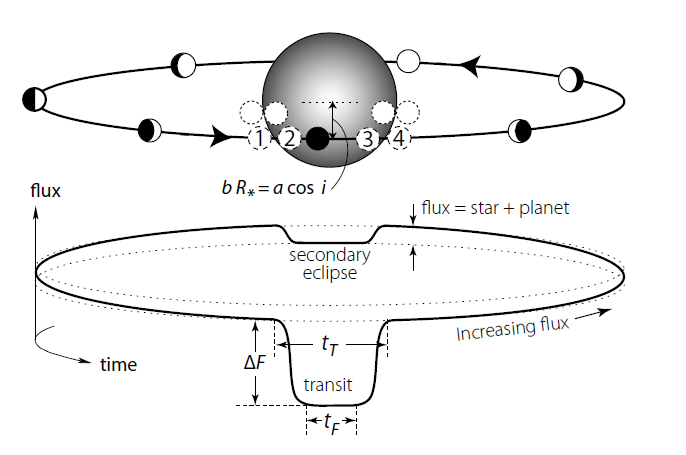
\includegraphics[width=0.6\linewidth]{TransitDarstellung.jpg}
		\caption{Schematische Darstellung eines Exoplaneten Transits und grundlegende Größen \cite{ExoHand}}
		\label{Abbildung 4.1}
	\end{figure}
	
	In Abbildung \ref{Abbildung 4.1} ist das Transit-Verfahren nochmals dargestellt. Die vier entscheidenden Größen des Transits sind dabei: die Periode $\mathcal{P}$, die Transittiefe $\Delta F$, sowie das Intervall zwischen dem ersten und vierten Kontakt $t_T$ und dem zweiten und dritten Kontakt $t_F$.  \\
	Mithilfe geometrischer Überlegungen folgen dann aus diesen Größen drei Gleichungen, die mitunter Aufschluss auf Planetenradius und Planetenbahn geben \cite{ExoHand}: 
	
	\begin{align} \label{Gleichung 4.1}
		\Delta F &\simeq \left( \frac{R_P}{R_\star} \right)^2 \\
		\sin\left( t_T \pi / \mathcal{P} \right) &= \frac{R_\star}{a} 
		\left\{ \frac{\left(1 + R_P / R_\star\right)^2 - \left( \left( a / R_\star \right) \cos i\right)^2}
		{1- \cos^2i} \right\} \\
		\frac{\sin (t_F \pi / \mathcal{P})}{\sin(t_T \pi / \mathcal{P})} & =
		\frac{\left( \left( 1- (R_P / R_\star)\right)^2 - \left( (a/ R_\star)\cos i\right)^2  
			\right)^{1/2} }
		{\left( \left(1 + (R_P / R_\star) \right)^2 - \left( (a/ R_\star) \cos i \right)^2
			\right)^{1/2}}
	\end{align}
	
	Möchte man nun eine Transit-Lichtkurve modellieren, unterscheidet man zwischen drei Bereichen. Zunächst befindet sich der Planet außerhalb des Sichtfelds des Sterns und die Intensität sollte konstant sein. Außerdem wird die Transittiefe $\Delta F$ bei kompletter Verdunklung durch den Planet durch Gleichung \ref{Gleichung 4.1} beschrieben. Zuletzt gibt es noch eine Übergangsphase, in der nur eine teilweise Bedeckung durch den Planeten stattfindet. \\
	In Realität ist die Helligkeit des Sterns nicht homogen, sondern nimmt zum Rand hin ab, da man auf zunehmend kühlere Schichten blickt, siehe Abbildung \ref{Abbildung 4.2}. Daher erreicht die Helligkeit in der Mitte des Transits ein Minimum. Eine realistische Modellierung eines Exoplanet-Transits befindet sich in Abbildung \ref{Abbildung 4.3}. Dabei wurden verschiedene Werte für den lotgerechten Abstand zwischen dem Planeten und dem Zentrum des Muttersterns b verwendet, siehe Abbildung \ref{Abbildung 4.1}.
	
	\begin{figure}[h]
		\begin{minipage}[b]{.4\linewidth} % [b] => Ausrichtung an \caption
			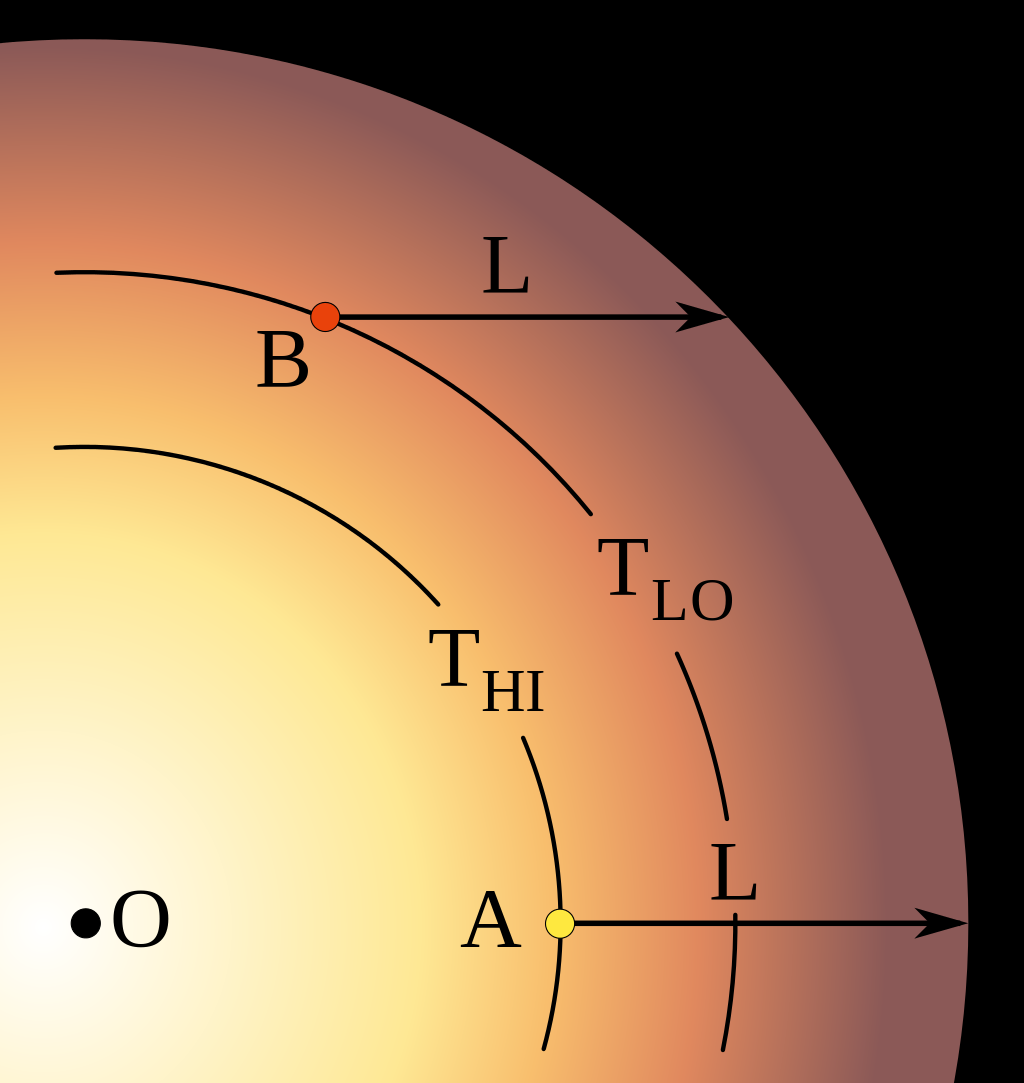
\includegraphics[width=\linewidth]{Limb_darkening_layers.svg.png}
			\caption{Randverdunklung eines Sterns \cite{wikiRand}}
			\label{Abbildung 4.2}
		\end{minipage}
		\hspace{.1\linewidth}% Abstand zwischen Bilder
		\begin{minipage}[b]{.4\linewidth} % [b] => Ausrichtung an \caption
			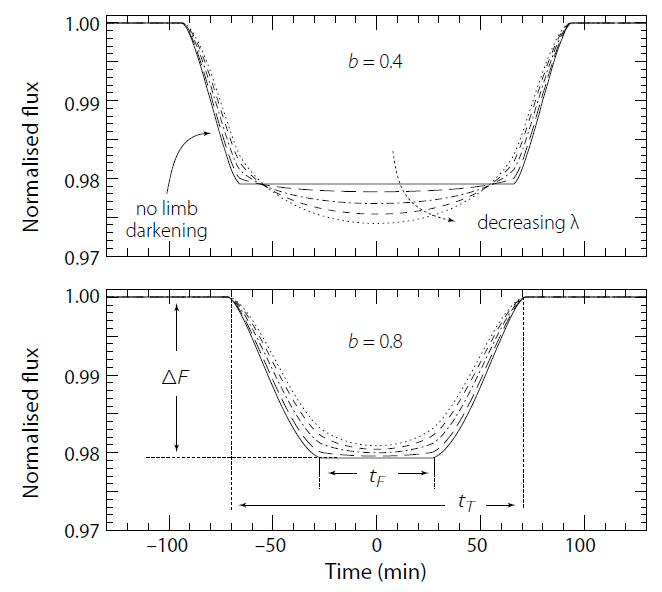
\includegraphics[width=\linewidth]{ModellExoLichtkurve.jpg}
			\caption{Beispielhafte Lichtkuven eines Exoplaneten Transits \cite{ExoHand}}
			\label{Abbildung 4.3}
		\end{minipage}
	\end{figure}
	
	\section{Objektauswahl}
	Für den Exoplaneten haben wir die Messdaten von einer anderen Gruppe übernommen. Zu analysieren ist der Planet HAT-P-12b, welcher in der Sternkonstellation Canes Venatici (Die Jagdhunde) zu finden ist. Das Kürzel für dieses Sternbild ist CVn und es befindet sich etwas südlich des Großen Wagens. 
	Aufgenommen wurden die Daten an dem 09.05.2024 zwischen 22 Uhr und 2:26 Uhr, mit einer Belichtungszeit von $60\si{s}$. Als Filter wurde nur der Luminanz-Filter verwendet. Das Teleskop CDK17, welches verwendet wurde, ist das größere der beiden Teleskope des TURMX Observatoriums. 
	Der Planet hat etwa eine Masse von 0.719±0.016 Jupitermassen und einen Radius von 0.7084±0.0095 Jupiterradien.
	Die äquatorialen Koordianten sind: RA 13 57 33.684 und DE +43 29 37.35 \cite{exoDataCzech}	\\
	
	
	\section{Photometrische Auswertung}
	
	Zur photometrischen Analyse wurde die Open-Source Software Muniwin des Software-Pakets \glqq C-Munipack \grqq benutzt, welche häufig in der Astronomie Verwendung findet. Dort wurden die Rohaufnahmen zunächst kalibriert mithilfe von in früheren Messungen aufgenommenen MasterDark und MasterFlat Bilder. Die anschließende photometrische Auswertung wird nun im Folgenden beschrieben.
	
	\subsection{Quick-Photometrie und Unsicherheit}
	Für eine anschließende Diskussion der Fehler, führen wir zunächst mit den Rohbilder (nicht kalibriert) eine  Quick-Photometrie durch und prüfen, ob die vom Programm berechneten Unsicherheiten mit denen in Abschnitt \ref{Subsec 2.3.2} theoretisch hergeleiteten Formel für die Unsicherheit übereinstimmen. \\
	Um den Fehler des Himmelshintergrund zu minimieren, verwenden wir die oben beschriebene Aperturphotometrie. Anhand der Abbildung \ref{Abbildung 4.4} kann man den Aperturradius, die Radien der Ringe, die Pixelanzahl und die ADUs ablesen. Anhand dieser Daten lässt sich das Gesamtsignal nach Gleichung \ref{Gleichung 2.4} und die Unsicherheit nach Gleichung \ref{Gleichung 2.6} bestimmen. 
	Da wir die Ringe so legen, dass keine anderen Sterne eingeschlossen werden, betrachten wir nur das Schrot- und Ausleserauschen.
	
	\begin{figure}[h]
		\centering
		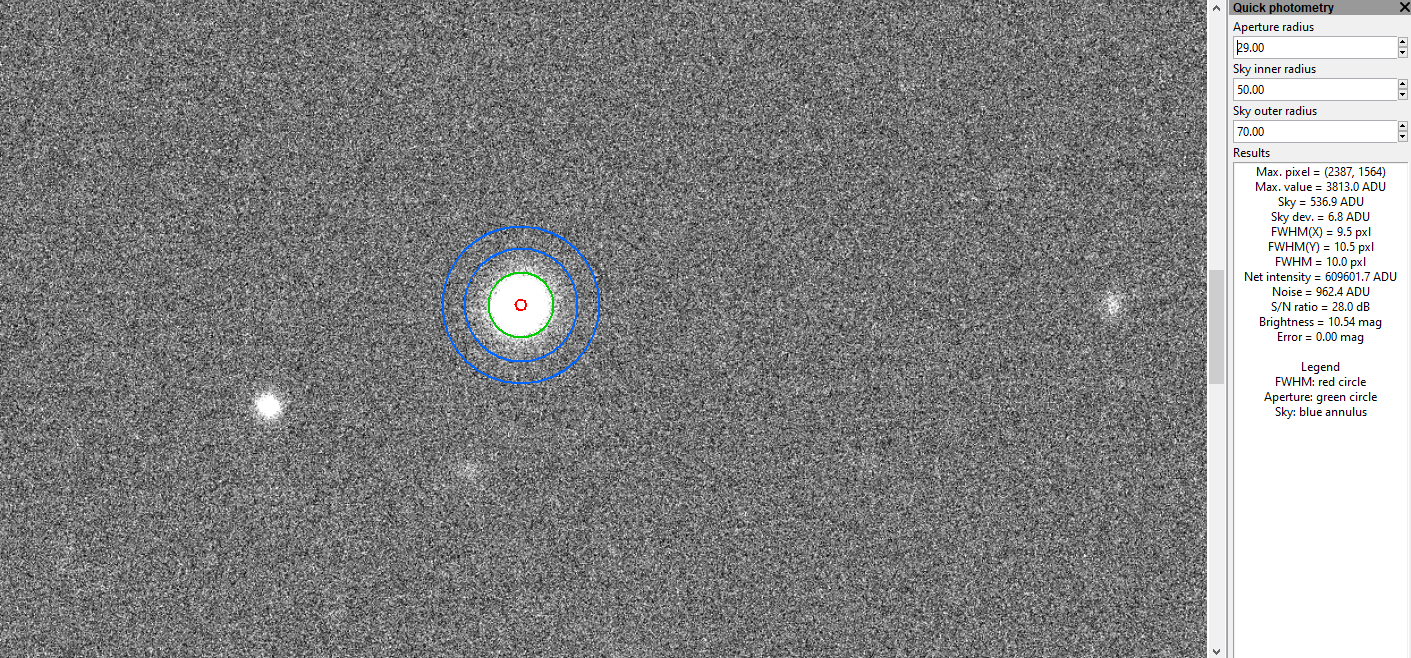
\includegraphics[width=0.8\linewidth]{Quick_Photometry_Fehler.PNG}
		\caption{Apertur Exoplanet und Fehler}
		\label{Abbildung 4.41}
	\end{figure}
	
	Die Unsicherheit des Gesamtsignals lässt sich anhand der Gleichung \ref{Gleichung 2.6} berechnen. Mit dem Aperturradius $R_A = 29\si{pxl}$, dem Innenradius $R_i = 50 \si{pxl}$ und Außenradius $R_o = 70 \si{pxl}$ lassen sich $A_A$, sowie $A_R$ berechnen. Außerdem kann anhand der Nettozählrate $\Sigma_N = 6ß9501 \si{ADU}$ und der Zählrate des Hintergrunds $\Sigma_R = 536,9\si{ADU}$ die Gesamtzählrate $\Sigma_A$ des Sterns und somit letztlich die Unsicherheit ermittelt werden. Es folgt:
	
	\begin{equation}
		\begin{aligned}
			\Delta \Sigma &= \cdot \sqrt{(g \cdot 3,5 e^-)^2 \cdot A_A \cdot (1 + A_A /A_R) + g \cdot \left( 
				\Sigma_A + \frac{A_A}{A_R}^2 \Sigma_R
				\right)} = 911,62 \si{ADU} \\
			\text{wobei}
			\quad
			A_A &= \pi R_A ^2 \si{pxl}= 2642,08 \si{pxl} 
			\quad 
			\text{und} 
			\quad
			A_R = \pi \cdot (R_o ^2 - R_i^2) \si{pxl} = 7539,82 \si{pxl} \\
			\text{sowie}
			\quad
			\Sigma_A &= 610137,9 \si{ADU} 
			\quad
			\text{und}
			\quad
			\Sigma_R = 536,9 \si{ADU}
		\end{aligned}
	\end{equation}
	Dieses Ergebnis entspricht der vom Programm berechneten Unsicherheit zu einer Genauigkeit von 5\%. Dies ist wahrscheinlich dem geschuldet, dass das Programm eine andere Rechnung verwendet, sowie keine Informationen über den Gain-Faktor g besitzt. Im Rahmen unseres Experiments stellt dies dennoch eine in Kauf nehmbare Abweichung dar.  
	
	\subsection{Vergleichs- und Checksterne} \label{Section 4.3.2}
	Da wir differenzielle Photometrie betreiben benötigen wir zur Berechnung des relativen Strahlungsflusses Vergleichs- und Checksterne. Muniwin detektiert dabei alle Sterne auf den Aufnahmen, die mindestens einen \glqq Minimum brightness – Detection threshold \grqq von 5 aufweisen. So wurden in jedem Bild circa 30 bis 40 Sterne identifiziert. Mithilfe des Web-Tools SIMBAD konnte durch Vergleich der Sternpositionen der Beobachtungsstern HAT-P-12b identifiziert werden. Die Vergleichs und Checksterne wurden so gewählt, dass diese sich einerseits relativ mittig im Bild befinden und andererseits eine konstante Lichtkurve aufweise, also selbst keine Veränderlichen sind. \\
	\begin{figure}[h!]
		\centering
		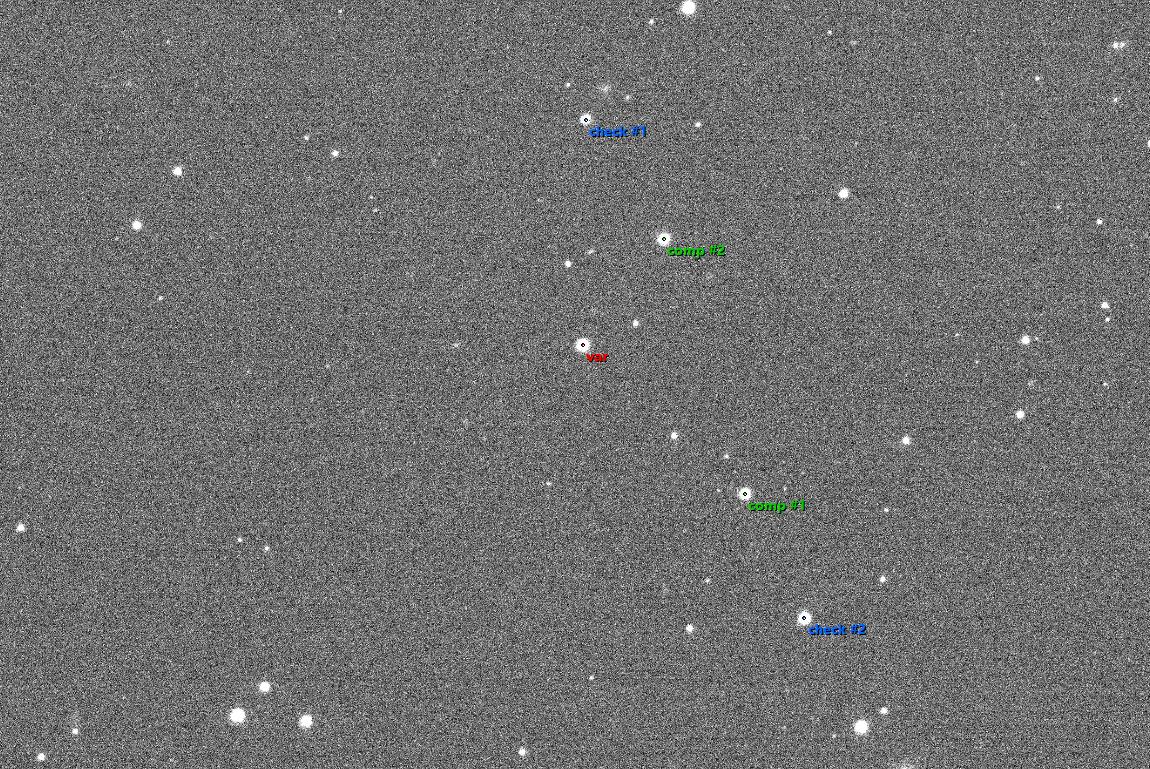
\includegraphics[width=0.8\linewidth]{VarCheckComp_exo.png}
		\caption{HAT-P-12, sowie Vergleichs- und Checksterne in einer Aufnahme}
		\label{Abbildung 4.5}
	\end{figure}
	
	\subsection{Modellierung der Lichtkurve}
	Zur Modellierung der Lichtkurve soll vereinfacht ein Trapezfit Verwendung finden, der an unsere Daten angepasst wurde. Mithilfe des Python Modules Scipy wurde dann die Parameter des Fits optimiert anhand unserer Daten. Mithilfe der Fit-Parameter können nun die physikalischen Parameter des Transits berechnet werden. Abbildung \ref{Abbildung 4.6} zeigt die gefittete Lichtkurve, wobei das Verhältnis der Strahlungsflüsse $S_V / S_C$ auf der y-Achse gegenüber der Zeit in julianischen Datum auf der x-Achse aufgetragen ist. 
	
	\begin{figure}[h!]
		\centering
		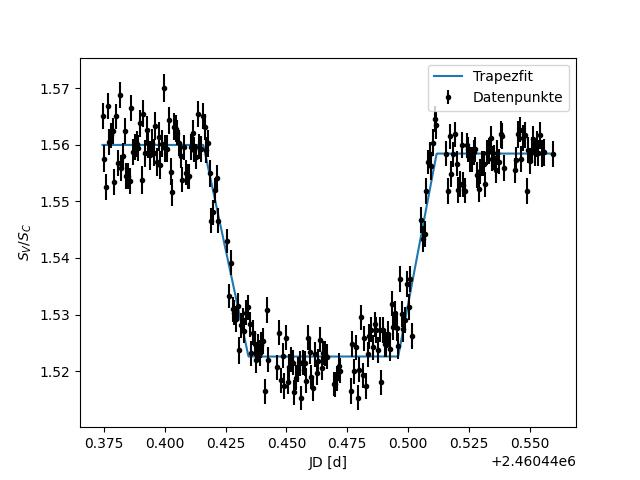
\includegraphics{Exoplanet_Trapez_Fit.jpg}
		\caption{Lichtkurve des Transits des Exoplaneten HAT-P-12b am 09.05.2024. Aufgetragen ist der relative Strahlungsfluss $S_V / S_C$ der Sonne HAT-P-12 und der Vergleichssternen über der Zeit im julianischen Datum.}
		\label{Abbildung 4.6}
	\end{figure}
	
	Man findet anhand der Modellierungsdaten folgende Parameter des Transits:
	
	\begin{itemize}
		\item \textbf{Transittiefe}\\
		Für die Transittiefe verwenden wir die konstanten Abschnitte des Transits und erhalten: 
		\begin{equation}
			\Delta F = 2,5 \cdot \left(\log\left(\left(\frac{S_V}{S_C}\right)_1\right) - \log\left(\left(\frac{S_V}{S_C}\right)_2\right)\right) = 0,0258(5) \si{mag}
		\end{equation}
		In dem Paper von Hartmann et. al. \cite{hartman2009hat} aus dem Jahr 2009 über die Entdeckung von HAT-P-12b wird eine Transittiefe von 2,5\% angegeben, was umgerechnet $0,027 \si{mag}$ entspricht. Die Abweichung von unserem Wert beträgt damit unter 5\%. Außerdem ist anzumerken, dass wir ein vereinfachtes Modell ohne Randverdunklung zum Kurvenfit verwendet haben, die Daten aber sehr wohl eine Randverdunklung nahelegen, siehe Abbildung \ref{Abbildung 4.6}.  
		\item \textbf{Transitdauer} \\
		Die Transitdauer ergibt sich aus der Zeitspanne des Einbruchs im Lichtkurvendiagramm.
		Unsere Daten ergeben: 
		\begin{equation}
			t_T = 138(4)\si{min}      
		\end{equation}
		In der \glqq Exoplanet Transit Database\grqq \cite{exoDataCzech} der Czech Astronomial Society ist für den Planeten HAT-P-12b eine Transitdauer von $140 \si{min}$ gelistet, was also im Rahmen der Unsicherheit unserem analysierten Wert entspricht. 
		\item \textbf{Totalitätsdauer}\\
		Auch interessant für den Transit ist die Zeitspanne, in der die Verdunklung durch den Planeten maximal und näherungsweise konstant ist. Diese war in unserem Modell gegeben durch:
		\begin{equation}
			t_t = 89(4) \si{min}
		\end{equation}
		\item \textbf{Transitmitte} \\
		Die Transitmitte ergibt sich zu:
		\begin{equation}
			\overline{t} = 2460440,4559(13) \si{JD}
		\end{equation}
		In der \glqq Exoplanet Transit Database\grqq \cite{exoDataCzech} der Czech Astronomial Society ist für den Planeten HAT-P-12b die Transitmitte für die geographischen Koordinaten des Telekeskops mit $\overline{t}_{\text{lit}} = 2460440,466 \si{JD}$ angegeben, was einer Differenz von 12 Minuten entspricht. Dies ist wahrscheinlich auf die Auswertung zurückzuführen, da der Einfachheit halber angenommen wurde, dass die Transitmitte in der Mitte der Totalitätsdauer stattfand. 
		\item \textbf{Verhältnis der Radien} \\
		Letztlich einfach aus den bereits ausgewerteten Daten lässt sich noch das Verhältnis der Radien des Planeten $R_P$ zur Sonne $R_S$ berechnen. Es gilt:
		\begin{equation}
			\frac{R_P}{R_S} = \sqrt{1 - \left( \frac{(S_V / S_C)_1}{(S_V / S_C)_2}\right)} = 0,1533(16)
		\end{equation}
		In Hartman et. al. \cite{hartman2009hat} ist ein Verhältnis von $R_P / R_S = 0.1406(13)$ gelistet, was zwar nicht innerhalb der Unsicherheit mit unseren Daten kompatibel ist (Abweichung 6\%), aber unter der Tatsache, dass wie ein vereinfachtes Modell ohne Randverdunklung gewählt haben, doch eine gute Näherung.  
	\end{itemize}
	\subsection{Andere Variablen}
	Das Programm Muniwin hat zusätzlich das Feature, automatisiert nach weiteren Variablen in den Bilder zu suchen. Allerdings hat sich die Suche bei unseren Daten als nicht erfolgreich herausgestellt. Alle weiteren Sterne wiesen geringere Helligkeitsvariationen auf, weshalb darauf zu schließen ist, dass höchstwahrscheinlich keine weiteren Variablen in unseren Daten zu finden sind. 
	
	
	
	\chapter{Veränderlicher Stern} 
	
	\subsection{Objektauswahl} 
	Wir haben den veränderlichen Stern ZTF J165048.86+152044.3 der Herkules Konstellation in der Nacht vom 30.06.2024 zwischen 22 und 3 Uhr untersucht.
Dieser Stern ist ein pulsierenden veränderlichen der HADS (High Amplitude δ Scuti stars) Klasse. Es handelt sich um radiale Pulsatoren mit asymmetrischen Lichtkurven, also steil ansteigende Zweige nd Amplituden >0,15 mag.
Dieser hat einer periodendauer von 75.14 Minuten und eine Magnituden range von 13.206 (0.202) g. Die Magnituden Range gibt die Schwankung der Helligkeit des Sterns an. Dabei sind die 13.206 die Durschnittshelligkeit und (0.202) die Standardabweichung. g steht für das g-band im Hertzsprung-Russel-Diagramm und gibt einen spezifischen Bereich des sichtbaren Lichtspektrums bei etwa 477 nm an.
Die Aufnahmen wurden mit einer Belichtungszeit von $120\si{s}$ und einem Luminanz-Filter aufgenommen.
	
	\subsection{Apertur-Photometrie}
	Analog zu dem Exoplaneten führen wir auch hier wieder eine Diskussion der Fehler mit den kalibrierten Rohbildern durch.
	
	\begin{figure}[h]
		\centering
		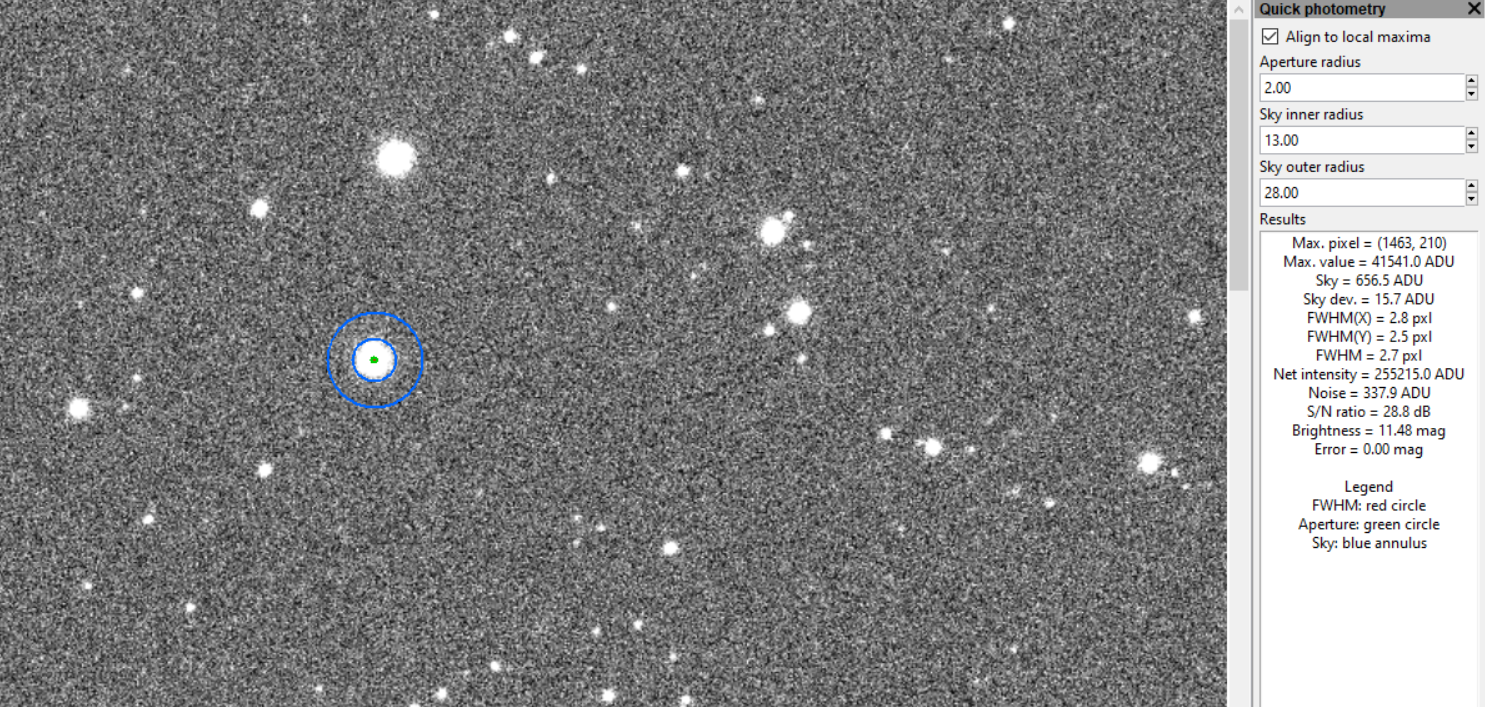
\includegraphics[width=0.8\linewidth]{Screenshot 2024-07-01 203800.png}
		\caption{Apertur veränderlicher Stern und Fehler}
		\label{Abbildung 4.42}
	\end{figure}
	
	Die Unsicherheit des Gesamtsignals lässt sich wieder anhand der Gleichung \ref{Gleichung 2.6} berechnen. Mit dem Aperturradius $R_A = 2\si{pxl}$, dem Innenradius $R_i =  13\si{pxl}$ und Außenradius $R_o =  28\si{pxl}$ lassen sich $A_A$ und $A_R$ berechnen. Außerdem kann anhand der Nettozählrate $\Sigma_N =  255215\si{ADU}$ und der Zählrate des Hintergrunds $\Sigma_R = 656.5\si{ADU}$ die Gesamtzählrate $\Sigma_A$ des Sterns und somit die Unsicherheit ermittelt werden. Es folgt:
	
	\begin{equation}
		\begin{aligned}
			\Delta \Sigma &= \cdot \sqrt{(g \cdot 3,5 e^-)^2 \cdot A_A \cdot (1 + A_A /A_R) + g \cdot \left( 
				\Sigma_A + \frac{A_A}{A_R}^2 \Sigma_R
				\right)} = ? \si{ADU} \\
			\text{wobei}
			\quad
			A_A &= \pi R_A ^2 \si{pxl}= 12,566 \si{pxl} 
			\quad 
			\text{und} 
			\quad
			A_R = \pi \cdot (R_o ^2 - R_i^2) \si{pxl} = 1932,08 \si{pxl} \\
			\text{sowie}
			\quad
			\Sigma_A &= ? \si{ADU} 
			\quad
			\text{und}
			\quad
			\Sigma_R = 656.5
			\si{ADU}
		\end{aligned}
	\end{equation}
	Dieses Ergebnis entspricht der vom Programm berechneten Unsicherheit zu einer Genauigkeit von ?\%. 
	
	\subsection{Vergleichs- und Check-Sterne}
	Die Vergleichssterne für die photometrische Auswertung werden nach dem Kapitel 4.3.2 beschriebenen Verfahren ausgewählt. Dabei konnte Der Stern mithilfe des Programms Simbad idetifiziert werden, und ist auf folgender Grafik rot makiert. Die Vergleichssterne (comp) sind grün und die Checksterne (Check) blau.
	
	\begin{figure}[h]
		\centering
		\includegraphics[width=0.8\linewidth]{entgültig.png}
		\caption{Vergleichs- und Checksterne}
		\label{Abbildung 4.43}
	\end{figure}
	
	



	\subsection{Rohdaten der Lichtkurve}
	Auf der Grundlage der Auswahl der Vergleichs- und Checksterne wurde die Magnitudendifferenz V-C gegen die Zeit des julianischen Datums JD geplottet.
	
	\begin{figure}[h]
		\centering
		\includegraphics[width=0.8\linewidth]{Endgültig.png}
		\caption{Lichtkurve}
		\label{Abbildung 4.44}
	\end{figure}

	Es konnte keine konstante Lichtkurve geplottet werden. Grund dafür ist unter anderem, dass sopwohl die vergleichssterne, als auch die Checksterne weit von dem zu unterscuhenden entfernt sind. Zudem weisen auch zwei der Comp-sterne veränderungen in ihrer Kurve auf. Einen weiteren Einfluss könnte sein, dass der Stern an verschiedenen Postionen am Nachthimmel ist.
Dennoch zeigt die Lichtkurve in der Abbildung eine schnelle Aufhellung, gefolgt von einem langsamen Abfall. Dies entspricht einer asymmetrischen Lichtkurve was für einen radialen Pulsator üblich ist. Dabei nimmt die amplitude mit der zeit größere Werte an, was allerdings untypisch ist.

	\subsection{Modellierung der Lichtkurve}
	Für die Modellierung der Lichtkurve verwenden wir einen Fourier-Reihen Fit bis zu einer bestimmten Abbruchsordnung Kmax. Aus diesen Daten wollen wir die Periodendauer, sowie die Magnitudenvariation bestimmen.
	Für Kmax wurde 25 gewählt, da diese schon gut mit den Messdaten übereinstimmen.

	\begin{figure}[h]
		\centering
		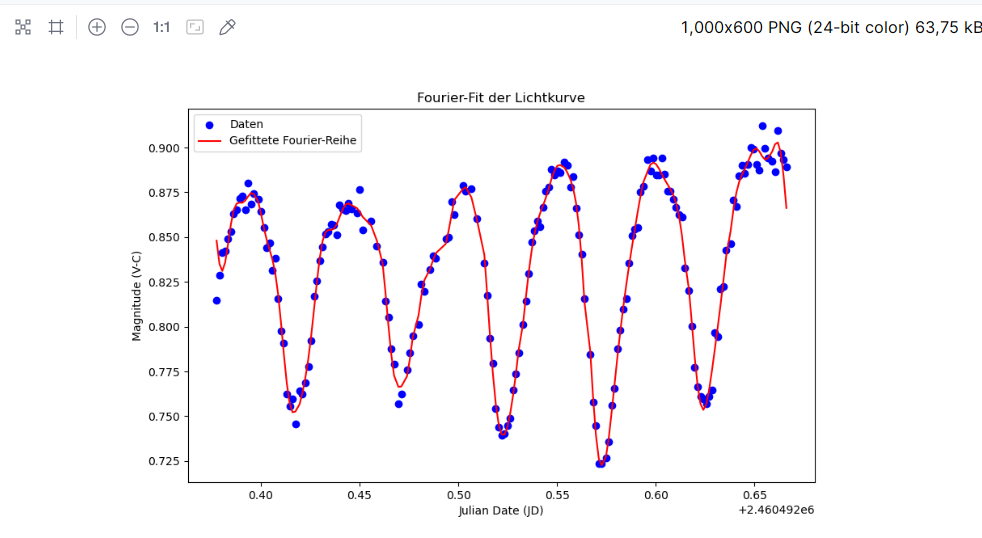
\includegraphics[width=0.8\linewidth]{LK_Fit}
		\caption{Lichtkurve}
		\label{Abbildung 4.44}
	\end{figure}

Die fourier-Koeffizienten wurden ermittelt zu:
\documentclass{article}
\usepackage{booktabs}

\begin{table}[ht]
    \centering
    \begin{tabular}{lccclcc}
        \toprule
        & \multicolumn{2}{c}{Koeffizient \( C \)} & & & \multicolumn{2}{c}{Koeffizient \( D \)} \\
        \cmidrule{2-3} \cmidrule{6-7}
        & Wert & Unsicherheit & & & Wert & Unsicherheit \\
        \midrule
        C1 & 148.3544439426628 & 0.6584042598265973 & & D1 & 0.0 & 0.0 \\
        C2 & 1.4797316268293592 & 0.45217539940824353 & & D2 & 0.566940771873932 & 0.46622344950367955 \\
        C3 & 0.8364302092998285 & 0.46218426850262656 & & D3 & 0.35810474319343094 & 0.46107919755197385 \\
        C4 & 1.1468796423098384 & 0.4383302432718888 & & D4 & 0.7321631581345506 & 0.46093453509558363 \\
        C5 & 2.0436985101608833 & 0.45980533763112685 & & D5 & -0.5814854340086469 & 0.44958824152211996 \\
        C6 & 0.836362743573689 & 0.4654889560181339 & & D6 & 1.9882055793482172 & 0.4624782012028237 \\
        C7 & -4.027492330174196 & 0.46644117890049747 & & D7 & -1.5211650054306496 & 0.4660644945621699 \\
        C8 & -0.10740873167461619 & 0.46093413898445795 & & D8 & 0.9303634821615013 & 0.4551137660223803 \\
        C9 & -0.1298747826343872 & 0.4546486802867936 & & D9 & -0.1933836696328291 & 0.4608624258445787 \\
        C10 & -0.3605492201411149 & 0.4671953830051102 & & D10 & 0.21013542233636115 & 0.4493068569196146 \\
        C11 & 1.1137123666049429 & 0.4539946222207847 & & D11 & 0.38103212093421784 & 0.4603165223333752 \\
        C12 & -0.3507638528367353 & 0.4422932435014157 & & D12 & 0.5284042296557919 & 0.45291404500540583 \\
        C13 & -0.1417280428956056 & 0.45356397130597054 & & D13 & -0.3958312535474161 & 0.44736799833733343 \\
        C14 & -0.5272265423748487 & 0.463807597841296 & & D14 & 0.3638324806716155 & 0.4360676594637262 \\
        C15 & -0.028568415980470767 & 0.46551720663099316 & & D15 & 0.22648257639744504 & 0.4651612268936313 \\
        C16 & 0.11313543797015604 & 0.4621966761427097 & & D16 & -0.12448025769161028 & 0.44914996515949135 \\
        C17 & -0.07118165550140172 & 0.4666724984605514 & & D17 & 0.490593449113487 & 0.4661874204314783 \\
        C18 & -0.03723818897021762 & 0.47294989905737667 & & D18 & 0.07486225032453828 & 0.4532527633061108 \\
        C19 & -0.12283619271543404 & 0.4588974511077617 & & D19 & -0.07114411995603849 & 0.44875592631660105 \\
        C20 & -0.025131187518731266 & 0.4455703033284666 & & D20 & 0.1842014241455037 & 0.44276876300859896 \\
        \bottomrule
    \end{tabular}
    \caption{Gefittete Koeffizienten \( C \) und \( D \) mit Unsicherheiten}
    \label{tab:gefittete_koeffizienten_cd}
\end{table}

Die Mittelwertbildung der Koeffizienten ergibt die Periodendauer T=(0.04809 ± 0.0012)d

Die ermittleten Daten werden mit denen aus dem Referenz-Katalog verglichen: T = 0.05, ∆VC >0.15mag
 Die ermittelte Periode weicht um 3,82 Prozent vom Literaturwert ab und die ermittelte
 Magnitudendifferenz weicht um ? ab. Die Abweichungen sind relativ groß, dies könnte auf die verschiedene Bedingungen zurückführbar sein, wie z.B: verschiedene Vergleichssterne, Messgeräte, Wetterbedingungen, Temperatur, etc..


	\chapter{Fazit}
	Wir konnten die Transittiefe, Transitdauer, Totalitätsdauer und Transitmitte von dem Exoplaneten HAT-P-12b bestimmen.
Der veränderliche Stern ZTF J165048.86+152044.3 konnte als pulsierender veränderlicher identifiziert werden. Ebenfalls konnte seine Periodendauer, sowie seine Magnitudendifferenz bestimmt werden.

	
	
	\printbibliography
	
	
\end{document}

